\documentclass[conference]{IEEEtran}
\IEEEoverridecommandlockouts

\usepackage{cite}
\usepackage{amsmath,amssymb,amsfonts}
\usepackage{graphicx}
\usepackage{booktabs}
\usepackage{array}
\usepackage{url}
\usepackage{xcolor}
\usepackage{tikz}
\usetikzlibrary{arrows.meta,positioning}

% Figures are read straight from the pipeline's output folder.
\graphicspath{{../reports/figures/}}

\begin{document}

\title{An Interpretable and Imbalance-Aware Machine Learning Framework for Road Accident Severity Prediction}

\author{\IEEEauthorblockN{Vansh Shetty}
\IEEEauthorblockA{\textit{Department of Computer Applications (MCA)} \\
\textit{NMAM Institute of Technology, Nitte (Deemed to be University)}\\
Nitte, Karnataka, India}}

\maketitle

\begin{abstract}
Machine learning (ML) studies of road accident severity are often limited to one region, report accuracy on imbalanced data, and sometimes leak information from test data or outcome attributes. This paper presents and evaluates a framework that addresses these gaps on Indian data. A panel of 11,752 State/UT $\times$ category $\times$ year rows was compiled from the Ministry of Road Transport and Highways (MoRTH) reports for 2019--2024 and validated against the published national totals. Decision Tree, AdaBoost, k-Nearest Neighbours and Categorical Naive Bayes, with a Random Forest as reference, are compared under three imbalance strategies in a leakage-safe protocol that trains on 2019--2022 and tests on 2023--2024. The four models reach test macro-F1 between 0.707 and 0.730 in their selected configurations (Random Forest 0.778), against 0.191 for a majority-class baseline; class weighting and SMOTEN change macro-F1 by at most 0.046. A Friedman test on repeated grouped cross-validation is significant ($\chi^2 = 13.200$, $p = 0.010$), but the Nemenyi test separates only Random Forest from AdaBoost. Macro-F1 falls from 0.750 to 0.410 when whole States are held out and rises to 0.981 when the severity index is leaked. Explanations agree that the State, not the crash condition, carries most of the signal. The framework is delivered as a web application with a risk check and a State-level map.
\end{abstract}

\begin{IEEEkeywords}
road safety, accident severity prediction, machine learning, class imbalance, data leakage, explainable AI, decision tree, AdaBoost
\end{IEEEkeywords}

% =====================================================================
\section{Introduction}

The World Health Organization estimates about 1.19 million road traffic deaths in 2021 \cite{who2023}, and India alone recorded 4,61,312 road accidents and 1,68,491 deaths in 2022 \cite{morth2022}. Knowing where, and under which road, environmental and vehicle conditions, accidents are most likely to be deadly can support proactive measures such as redesigning junctions or prioritising emergency resources.

ML models can learn such relationships from historical records \cite{behboudi2024}, but their usefulness depends on how they are built and evaluated. When severity classes are imbalanced, a model that always predicts the most common class can appear accurate while being useless. Evaluation pipelines can also leak information, for example by oversampling before splitting the data or by including attributes computed from the outcome, a well-documented cause of irreproducible results \cite{kapoor2023}.

In India, crash data are published openly only as aggregate tables in the annual MoRTH reports. This paper therefore applies the framework at the level at which the data exist: it predicts the severity level of a category of accidents (for example, accidents in fog) in a State or Union Territory (UT) in a year. Its contributions are:
\begin{itemize}
\item a validated, machine-readable panel of MoRTH accident statistics for 2019--2024, with every correction logged;
\item a comparison of Decision Tree (DT), AdaBoost, k-Nearest Neighbours (KNN) and Naive Bayes (NB), with a Random Forest (RF) as reference, under one leakage-safe protocol with three imbalance strategies, a majority-class baseline and significance tests;
\item a generalisability test on held-out States, a leakage audit and an explainability layer of rules and feature attribution;
\item a web tool with severity prediction and a State-level map.
\end{itemize}

Section~\ref{sec:related} reviews related work; Sections~\ref{sec:architecture} and~\ref{sec:implementation} present the architecture and implementation; Section~\ref{sec:dataset} the dataset; Section~\ref{sec:discussion} the outcomes; Sections~\ref{sec:method} and~\ref{sec:evaluation} the methodology and evaluation design; Section~\ref{sec:results} the results; Section~\ref{sec:conclusion} concludes.

% =====================================================================
\section{Related Work}
\label{sec:related}

Comparative studies dominate the crash-severity literature. Iranitalab and Khattak \cite{iranitalab2017} compared four statistical and ML methods on Nebraska data and showed that the evaluation criterion changes which method appears best. AlMamlook et al. \cite{almamlook2019} compared AdaBoost, logistic regression, NB and RF on Michigan data, and Shiran et al. \cite{shiran2021} compared multinomial logit, decision trees and neural networks. Al-Mistarehi et al. \cite{almistarehi2022} combined ML with GIS analysis in Jordan, and Mohamad et al. \cite{mohamad2025} evaluated eight algorithms on 112,837 crashes in Thailand. Other work studies RF alone \cite{hoanglong2021}, UK data \cite{vanitha2023} and Ethiopian records \cite{ethiopia2025}. Angarita-Zapata et al. \cite{angarita2021} benchmarked ML and AutoML in three Colombian cities, and Behboudi et al. \cite{behboudi2024} reviewed 191 studies.

\subsection{Research Gaps}
Five limitations recur: (1) models are validated on a single region; (2) studies favour either opaque ensembles or weaker interpretable models, rarely both under one protocol; (3) contextual data are under-used; (4) models remain offline artefacts; and (5) class imbalance is seldom addressed and results are summarised by accuracy.

\subsection{Research Questions}
\begin{itemize}
\item[RQ1] How do DT, AdaBoost, KNN and NB compare on macro-F1, balanced accuracy and High-class recall?
\item[RQ2] How much do class weighting and synthetic oversampling improve recall on the High-severity class?
\item[RQ3] Which factors most influence the severity level, and are they consistent across models?
\item[RQ4] Does a model keep its performance on States it was not trained on, and on later years?
\end{itemize}

% =====================================================================
\section{System Architecture}
\label{sec:architecture}

Fig.~\ref{fig:architecture} shows the five layers. The \emph{data sources} are the State and UT annexure tables of the MoRTH reports, plus a boundary file used only for mapping. In \emph{data processing} the tables are extracted and validated, and every fitted step runs inside a pipeline so that it is learnt from training data only. In the \emph{model layer} the classifiers are tuned under one protocol and selected by cross-validated macro-F1 on the training years. The \emph{insight layer} explains the models and, because the data carry no coordinates, maps severity by State. The \emph{application layer} serves the selected pipeline through a REST API and a web interface.

\begin{figure*}[t]
\centering
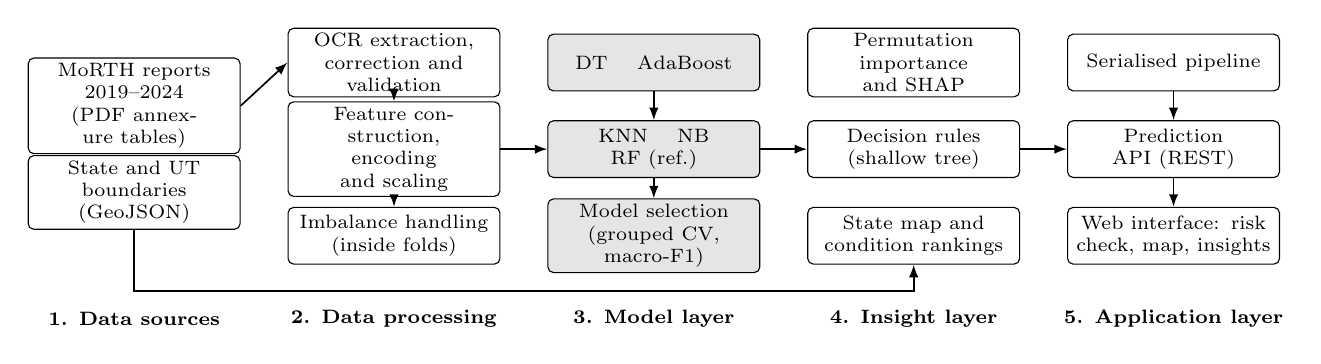
\begin{tikzpicture}[font=\scriptsize,
  box/.style={draw, rounded corners=2pt, align=center, text width=2.55cm, minimum height=0.72cm, inner sep=2pt},
  model/.style={box, fill=gray!20},
  arr/.style={-{Latex[length=1.6mm]}, semithick}]
\node[box] (s1) at (0,0.55) {MoRTH reports 2019--2024\\(PDF annexure tables)};
\node[box] (s2) at (0,-0.55) {State and UT boundaries\\(GeoJSON)};
\node[box] (p1) at (3.3,1.1) {OCR extraction,\\correction and validation};
\node[box] (p2) at (3.3,0) {Feature construction,\\encoding and scaling};
\node[box] (p3) at (3.3,-1.1) {Imbalance handling\\(inside folds)};
\node[model] (m1) at (6.6,1.1) {DT \quad AdaBoost};
\node[model] (m2) at (6.6,0) {KNN \quad NB \quad RF (ref.)};
\node[model] (m3) at (6.6,-1.1) {Model selection\\(grouped CV, macro-F1)};
\node[box] (i1) at (9.9,1.1) {Permutation importance\\and SHAP};
\node[box] (i2) at (9.9,0) {Decision rules\\(shallow tree)};
\node[box] (i3) at (9.9,-1.1) {State map and\\condition rankings};
\node[box] (u1) at (13.2,1.1) {Serialised pipeline};
\node[box] (u2) at (13.2,0) {Prediction API (REST)};
\node[box] (u3) at (13.2,-1.1) {Web interface: risk\\check, map, insights};
\draw[arr] (s1.east) -- (p1.west);
\draw[arr] (p1) -- (p2);
\draw[arr] (p2) -- (p3);
\draw[arr] (p2.east) -- (m2.west);
\draw[arr] (m1) -- (m2);
\draw[arr] (m2) -- (m3);
\draw[arr] (m2.east) -- (i2.west);
\draw[arr] (i2.east) -- (u2.west);
\draw[arr] (u1) -- (u2);
\draw[arr] (u2) -- (u3);
\draw[arr] (s2.south) |- (9.9,-1.8) -- (i3.south);
\node at (0,-2.15) {\textbf{1. Data sources}};
\node at (3.3,-2.15) {\textbf{2. Data processing}};
\node at (6.6,-2.15) {\textbf{3. Model layer}};
\node at (9.9,-2.15) {\textbf{4. Insight layer}};
\node at (13.2,-2.15) {\textbf{5. Application layer}};
\end{tikzpicture}
\caption{Five-layer system architecture. The model layer (shaded) is evaluated under the leakage-safe protocol of Section~\ref{sec:method}.}
\label{fig:architecture}
\end{figure*}

% =====================================================================
\section{Implementation}
\label{sec:implementation}

The framework is implemented in Python~3.11 with pandas, scikit-learn \cite{pedregosa2011}, imbalanced-learn \cite{lemaitre2017}, SHAP \cite{lundberg2017} and scikit-posthocs. The prediction service is a Flask REST API that validates every input, and the front end is a single page that uses Leaflet. One command runs the whole pipeline and regenerates every table and figure; the random seed is 42 throughout.
% AUTHOR: add the public repository URL here if the code is released.

% =====================================================================
\section{Dataset Description}
\label{sec:dataset}

\subsection{Source and Compilation}
The dataset is compiled from the annual MoRTH publication \emph{Road Accidents in India} \cite{morth2022,morthseries}, editions 2019 to 2024. Nine State- and UT-wise annexure tables are used, each a different breakdown of the same accidents: collision type, road environment, road feature, junction type, traffic control, weather, impacting vehicle, traffic violation and area type.

The annexures are printed tables inside PDF reports. Each page was rendered at 400~dpi, the table grid was located with OpenCV, and each column was read with Tesseract optical character recognition. A misread that broke a validation check was corrected only when the corrected value appears in the PDF's own text layer or is confirmed by a re-read of the cell or the printed page, and the check then passes. In total 79 cells were corrected, and every correction is logged. The result is a panel of 11,752 rows and 17 columns, in which one row is one State or UT, one factor value and one year. Two administrative units are merged or split during the period; a harmonised State attribute maps them to 35 comparable units.

\subsection{Validation}
Five checks were applied: (1) every column of every table sums to the All-India total printed in the report; (2) grievously injured plus minor injured equals total injured in every row; (3) six of the nine groups reproduce the national accidents, deaths and injuries in every year; (4) for those groups every State's sum equals its State total, except two differences that exist in MoRTH's printed 2020 tables (persons killed in Meghalaya, 6 more in the impacting-vehicle table, and in Tamil Nadu, 1 more in the road-feature table), which are kept as printed; and (5) the national totals match the published figures, from 449,002 accidents and 151,113 deaths in 2019 to 487,707 and 177,175 in 2024.

\subsection{Target, Features and Leakage Control}
MoRTH defines the severity index as persons killed per 100 accidents. The target, the \emph{severity level}, is Low if a row's index is below 0.75 times the national index of that year, High if above 1.25 times, and Medium otherwise. Rows with fewer than 10 accidents are excluded, leaving 9,332 rows from 34 States and UTs: 6,327 for training on 2019--2022 (1,968 Low, 1,952 Medium, 2,407 High) and 3,005 for testing on 2023--2024 (883, 913 and 1,209). The classes are only mildly imbalanced, and High is the largest class, not the rarest.

Seven features are used: factor group, factor value, region, State or UT status, harmonised State, year and $\log(1+\text{accidents})$. The numbers killed and injured, the severity index and the national severity define the target and are excluded.

\subsection{Coverage Changes Between Years}
Junction type and traffic control cover all accidents in 2019--2021 but only junction accidents from 2022 (20.1\% to 22.6\% of accidents), and road environment covers 41.2\% in 2024. Totals are therefore always taken from one group, collision type.

% =====================================================================
\section{Discussion: Outcomes}
\label{sec:discussion}

The study delivers: a reproducible benchmark of four classifiers against a majority-class baseline (Table~\ref{tab:test}); evidence that they are not statistically separable on held-out States (Fig.~\ref{fig:general}); quantified, small effects of imbalance handling; a leakage audit and evidence that performance does not transfer to unseen States (Fig.~\ref{fig:robust}); and explanations that agree that geography dominates, delivered in a working web application.

% =====================================================================
\section{Methodology}
\label{sec:method}

\subsection{Preprocessing}
For DT, AdaBoost, KNN and RF, categorical attributes are one-hot encoded and numeric ones standardised. For NB, attributes are ordinal-encoded and the accident count is discretised into quartile bins. A category unseen in training is encoded as all zeros, or for NB as a reserved code that contributes only the smoothing term.

\subsection{Classification Algorithms}
DT is a CART tree \cite{breiman1984} whose root-to-leaf paths form readable rules. AdaBoost \cite{freund1997} boosts depth-2 trees in its multi-class SAMME form. KNN \cite{cover1967} uses Euclidean distance on the encoded attributes. Categorical NB assumes conditional independence with Laplace smoothing. An RF \cite{breiman2001} of 300 trees is a reference against which the four are positioned.

\subsection{Imbalance Handling}
Three strategies are compared: no handling; class weighting, with weight $w_c = N/(K n_c)$ for a class with $n_c$ of $N$ rows and $K = 3$; and SMOTEN, the categorical variant of SMOTE \cite{chawla2002} based on the value difference metric \cite{stanfill1986}. AdaBoost receives the weights as sample weights and NB uses a uniform class prior; KNN has no class-weight mechanism, which leaves 14 pipelines. Resampling is applied only to the training part of each fold through an imbalanced-learn pipeline \cite{lemaitre2017}.

\subsection{Hyperparameter Tuning}
Grids are searched on the training years with 5-fold cross-validation grouped by State, maximising macro-F1: DT depth $\{4, 6, 10, \text{none}\}$ and minimum leaf $\{1, 5, 20\}$; AdaBoost $\{100, 300\}$ estimators and learning rate $\{0.1, 0.5, 1.0\}$; KNN $k \in \{5, 11, 21\}$ with uniform or distance weights; NB $\alpha \in \{0.1, 0.5, 1.0\}$; RF depth $\{10, \text{none}\}$ and minimum leaf $\{1, 5\}$. For each model, the strategy with the highest cross-validated macro-F1 is its \emph{selected configuration}; the test years play no part in this choice.

\subsection{Explainability}
Permutation importance (the drop in macro-F1 when an attribute is shuffled, 10 repeats) is computed on the test set for the best interpretable model. A shallow tree (depth 4, at least 30 rows per leaf, balanced weights) is trained and its rules are ranked by weighted relative accuracy. SHAP values \cite{lundberg2017} explain the best ensemble.

% =====================================================================
\section{Evaluation Design}
\label{sec:evaluation}

\subsection{Metrics}
The primary metrics are macro-F1 and balanced accuracy, which average per-class F1 and recall over the three classes, together with High-class recall. Accuracy and macro-averaged one-vs-rest ROC-AUC and precision--recall AUC are secondary. Every pipeline is scored once on the test years, next to a baseline that always predicts the most common training class.

\subsection{Statistical Comparison and Generalisability}
Each selected configuration is re-evaluated on the training years with grouped cross-validation (5 folds by State, repeated twice), all models on the same 10 folds. The Friedman test and the Nemenyi post-hoc test assess differences in average rank \cite{demsar2006}. Holding out whole States is also the test of generalisability across space; across time, the model trained on 2019--2022 is scored separately on 2023 and 2024.

\subsection{Leakage Audit}
Control experiments on the DT, with hyperparameters held at their tuned values, compare the leakage-safe setup with two pitfalls: a random row split that places a State on both sides, and the retention of an attribute that defines the target.

% =====================================================================
\section{Results}
\label{sec:results}

\subsection{Model Comparison and Baseline (RQ1)}
Table~\ref{tab:test} and Fig.~\ref{fig:models} report all 14 pipelines on the 3,005 test rows. The baseline, which always predicts High, reaches accuracy 0.402 but macro-F1 0.191 and balanced accuracy 0.333. Every pipeline is far above it, with macro-F1 from 0.687 to 0.778. In their selected configurations the four core models are close: KNN 0.730, AdaBoost 0.717, DT 0.711 and NB 0.707, with High recall 0.781, 0.733, 0.728 and 0.746. The reference RF is highest (macro-F1 0.778, High recall 0.792). The single highest High recall, 0.828, belongs to KNN without handling. \textbf{Answer to RQ1:} KNN ranks first among the four and NB last, but they are 0.023 apart in macro-F1, and RF is 0.048 above KNN.

\begin{table*}[t]
\caption{Test-Set Performance on the 2023--2024 Data ($n = 3{,}005$). AUCs Are One-vs-Rest, Macro-Averaged. Bold Marks the Best Pipeline in Each Column; $^\ast$ Marks Each Model's Selected Configuration; $^\dagger$ Reference Model Only.}
\label{tab:test}
\centering
\footnotesize
\setlength{\tabcolsep}{5pt}
\begin{tabular}{@{}llrrrrrrrr@{}}
\toprule
Model & Strategy & Accuracy & Bal.\ acc. & Macro-F1 & Recall Low & Recall Med. & Recall High & ROC-AUC & PR-AUC \\
\midrule
Majority baseline & Always High & 0.402 & 0.333 & 0.191 & 0.000 & 0.000 & 1.000 & 0.500 & 0.333 \\
\midrule
Decision Tree & None & 0.693 & 0.692 & 0.687 & 0.821 & 0.544 & 0.711 & 0.872 & 0.768 \\
Decision Tree & Class weights & 0.735 & 0.734 & 0.733 & 0.783 & 0.673 & 0.748 & 0.874 & 0.762 \\
Decision Tree$^\ast$ & SMOTEN & 0.716 & 0.716 & 0.711 & 0.822 & 0.597 & 0.728 & 0.858 & 0.738 \\
AdaBoost$^\ast$ & None & 0.719 & 0.718 & 0.717 & 0.776 & 0.645 & 0.733 & 0.868 & 0.762 \\
AdaBoost & Class weights & 0.714 & 0.720 & 0.716 & 0.796 & \textbf{0.694} & 0.668 & 0.867 & 0.752 \\
AdaBoost & SMOTEN & 0.720 & 0.720 & 0.719 & 0.777 & 0.660 & 0.723 & 0.869 & 0.752 \\
KNN & None & 0.753 & 0.746 & 0.744 & 0.844 & 0.567 & \textbf{0.828} & 0.886 & 0.792 \\
KNN$^\ast$ & SMOTEN & 0.737 & 0.733 & 0.730 & 0.830 & 0.588 & 0.781 & 0.883 & 0.785 \\
Naive Bayes & None & 0.716 & 0.710 & 0.707 & 0.802 & 0.551 & 0.778 & 0.875 & 0.770 \\
Naive Bayes$^\ast$ & Class weights & 0.712 & 0.709 & 0.707 & 0.800 & 0.582 & 0.746 & 0.875 & 0.771 \\
Naive Bayes & SMOTEN & 0.716 & 0.711 & 0.708 & 0.805 & 0.552 & 0.776 & 0.875 & 0.772 \\
\midrule
Random Forest$^\dagger$ & None & 0.747 & 0.745 & 0.742 & 0.828 & 0.627 & 0.779 & 0.898 & 0.811 \\
Random Forest$^{\dagger\ast}$ & Class weights & \textbf{0.781} & \textbf{0.781} & \textbf{0.778} & \textbf{0.866} & 0.686 & 0.792 & \textbf{0.920} & \textbf{0.848} \\
Random Forest$^\dagger$ & SMOTEN & 0.746 & 0.747 & 0.744 & 0.831 & 0.664 & 0.747 & 0.899 & 0.813 \\
\bottomrule
\end{tabular}
\end{table*}

\begin{figure}[t]
\centering
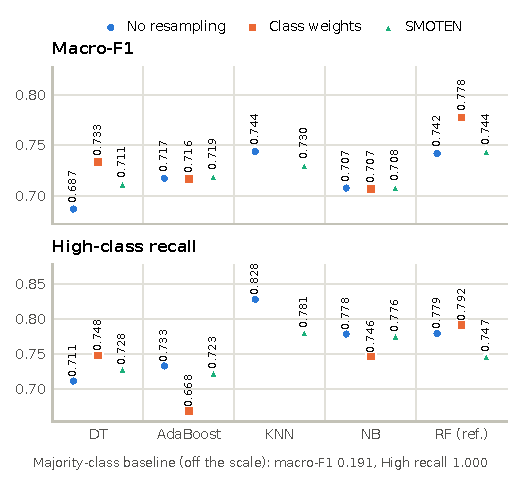
\includegraphics[width=0.95\columnwidth]{fig14_paper_model_comparison}
\caption{Test-set macro-F1 and High-class recall of the 14 pipelines. The vertical scales do not start at zero.}
\label{fig:models}
\end{figure}

\subsection{Imbalance Strategies (RQ2)}
Relative to no handling, class weighting changes High recall by $+0.036$ for DT, $-0.065$ for AdaBoost, $-0.032$ for NB and $+0.012$ for RF; SMOTEN changes it by $+0.017$ for DT, $-0.010$ for AdaBoost, $-0.047$ for KNN, $-0.002$ for NB and $-0.032$ for RF. Macro-F1 moves by at most 0.046 (DT with class weighting, 0.687 to 0.733). The gains are on the Medium class, whose recall rises with class weighting from 0.544 to 0.673 for DT and from 0.627 to 0.686 for RF. \textbf{Answer to RQ2:} High recall improves in three of nine cases, by at most 0.036, and falls in six, by up to 0.065. High is the largest class (38.0\% of training rows), so rebalancing moves predictions away from it.

\subsection{Statistical Comparison}
On the repeated grouped folds (Fig.~\ref{fig:general}) mean macro-F1 is 0.454 for RF, 0.447 for KNN, 0.425 for NB, 0.397 for DT and 0.380 for AdaBoost, with average ranks 2.0, 2.3, 2.9, 3.6 and 4.2. The Friedman test rejects equal performance ($\chi^2(4) = 13.200$, $p = 0.010$). The Nemenyi critical difference at $\alpha = 0.05$ is 1.929 ranks. Only RF against AdaBoost differs significantly ($p = 0.016$); KNN against AdaBoost is close ($p = 0.056$), and every other pair has $p \geq 0.157$. The four core models cannot be ranked with confidence on unseen States.

\begin{figure}[t]
\centering
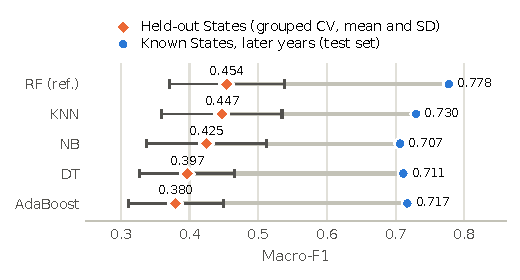
\includegraphics[width=0.95\columnwidth]{fig15_paper_generalisation}
\caption{Macro-F1 of each model's selected configuration on held-out States (5 folds $\times$ 2 repeats by State, 2019--2022) and on the 2023--2024 test set.}
\label{fig:general}
\end{figure}

\begin{figure}[t]
\centering
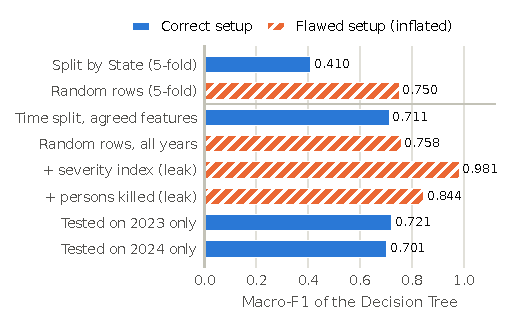
\includegraphics[width=0.95\columnwidth]{fig16_paper_robustness}
\caption{Control experiments on the Decision Tree (SMOTEN). The first two rows are cross-validated on 2019--2022; the others are scored on test years.}
\label{fig:robust}
\end{figure}

\subsection{Robustness and Leakage (RQ4)}
Fig.~\ref{fig:robust} reports the control experiments. With whole States held out the tree reaches macro-F1 0.410; a random split of the same rows reaches 0.750, an inflation of 0.340. The time split also has every State on both sides, which explains why its score (0.711) is close to the random split. Adding the severity index to the features lifts test macro-F1 to 0.981, and adding persons killed lifts it to 0.844. \textbf{Answer to RQ4:} performance does not transfer to unseen States: all five models score 0.380 to 0.454 in grouped cross-validation against 0.707 to 0.778 on the time split (Fig.~\ref{fig:general}). Over time the decline is small, from 0.721 on 2023 to 0.701 on 2024.

\begin{figure}[t]
\centering
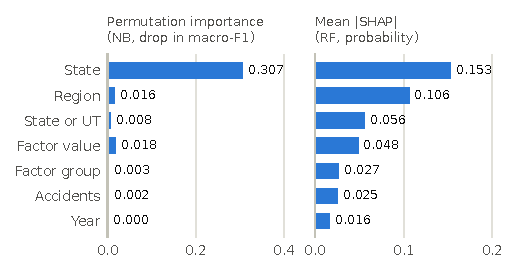
\includegraphics[width=0.95\columnwidth]{fig17_paper_importance}
\caption{Attribute importance under two methods: permutation importance for Naive Bayes on the test years, and mean absolute SHAP value for the Random Forest.}
\label{fig:importance}
\end{figure}

\subsection{Explainability (RQ3)}
Fig.~\ref{fig:importance} compares two attribution methods. For NB with class weighting, shuffling the State lowers test macro-F1 by 0.307, against 0.018 for the factor value, 0.016 for region and 0.008 or less for the other attributes. The shallow tree (test macro-F1 0.555) has 8 distinct rules, and its most useful ones are all geographic: outside the South, except three States, predict High (4,352 training rows, precision 0.537; test precision 0.570); in the South, except Andhra Pradesh and Telangana, predict Low (906 rows, 0.807; test 0.749). For RF with class weighting, the mean absolute SHAP value is 0.153 for State, 0.106 for region and 0.056 for State or UT status, ahead of the factor value (0.048). \textbf{Answer to RQ3:} the State is the most influential attribute under all three methods and for NB, DT and RF, followed by region; the crash condition has a real but much smaller influence.

\subsection{India Map and Insights}
From the dataset alone, national severity rose from 33.66 persons killed per 100 accidents in 2019 to 36.33 in 2024; over six years the panel records 2,657,174 accidents and 955,355 deaths (35.95). Fig.~\ref{fig:map} maps the States. Among those with at least 500 accidents, the highest values in 2024 are in Bihar (80.51), Jharkhand (79.18) and Punjab (78.49) and the lowest in Kerala (7.95) and Goa (10.66); the largest rises since 2019 are in Chhattisgarh ($+10.75$) and Tamil Nadu ($+8.93$). By region, severity ranges from 24.77 in the South to 59.76 in the East. The deadliest conditions nationally are hail or sleet (46.203), run-off-road (46.062), vehicle-overturn (45.821) and hit-and-run (45.330) accidents; hit and run alone accounts for 174,176 deaths.

\begin{figure*}[t]
\centering
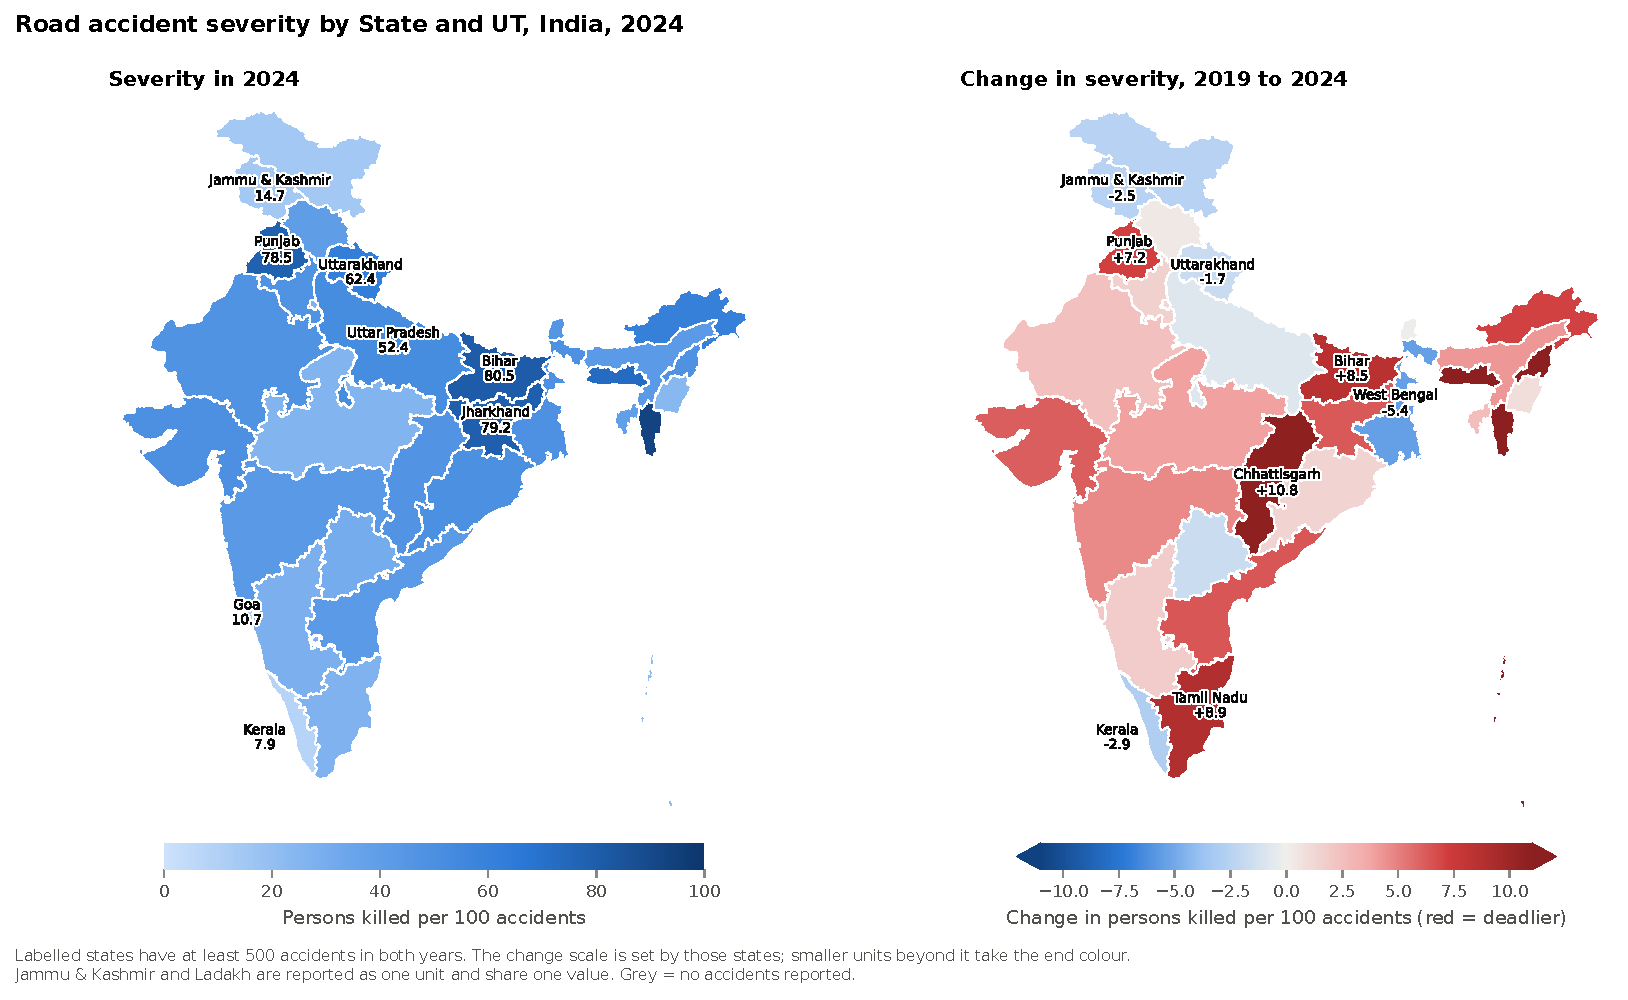
\includegraphics[width=0.62\textwidth]{fig11_state_severity_map}
\caption{Road accident severity (persons killed per 100 accidents) by State and UT in 2024, and the change from 2019.}
\label{fig:map}
\end{figure*}

\subsection{Web Application}
The risk check returns the predicted level, class probabilities, the three attributes with the largest SHAP contribution and the yearly record of the chosen State and condition. The map view shows Fig.~\ref{fig:map} for any year, and an insights view ranks the deadliest conditions. The application serves the pipeline with the highest tuning macro-F1, which is the reference RF.

\subsection{Limitations}
\emph{Aggregate data:} every row is a yearly total for a State and a category, so the models classify categories of accidents, not individual crashes, and combinations of conditions are not available. \emph{Time split:} the test years contain the same States as the training years, so the test scores describe known States only, and the drift estimate rests on two years. \emph{Category changes:} three factor groups do not cover the same accidents in every year (Section~\ref{sec:dataset}). In addition, the severity index depends on reporting practice; the classes are only mildly imbalanced, so the findings on imbalance handling should not be generalised to data with a rare severe class; the significance tests use folds that share data, so their $p$-values are approximate; and the SHAP analysis and application use the reference RF.

% =====================================================================
\section{Conclusion}
\label{sec:conclusion}

This paper has evaluated an interpretable, imbalance-aware and leakage-safe framework for road accident severity prediction on a validated panel of MoRTH statistics for 2019--2024. The four lightweight classifiers reach test macro-F1 between 0.707 and 0.730, against 0.191 for a majority-class baseline and 0.778 for the reference RF, and are not statistically separable on held-out States. Class weighting and SMOTEN change macro-F1 by at most 0.046, because High is the largest class in these data. The control experiments carry the main message: a random row split inflates macro-F1 by 0.340 over a split by State, and leaking the severity index raises it from 0.711 to 0.981. All three explanation methods agree that the State carries most of the signal, so the models describe where accidents are deadly far better than which conditions make them so. These conclusions are bounded by aggregate State-level data, a time split that shares States, and categories whose coverage changes. Future work will apply the framework to record-level Indian crash data and replace the State identifier with features that describe States directly.

\begin{thebibliography}{00}
\bibitem{who2023} World Health Organization, \emph{Global Status Report on Road Safety 2023}. Geneva, Switzerland: WHO, 2023.
\bibitem{morth2022} Ministry of Road Transport and Highways, Transport Research Wing, \emph{Road Accidents in India 2022}. New Delhi, India: Government of India, 2023.
\bibitem{behboudi2024} N. Behboudi, S. Moosavi, and R. Ramnath, ``Recent advances in traffic accident analysis and prediction: A comprehensive review of machine learning techniques,'' arXiv:2406.13968, 2024.
\bibitem{kapoor2023} S. Kapoor and A. Narayanan, ``Leakage and the reproducibility crisis in machine-learning-based science,'' \emph{Patterns}, vol. 4, no. 9, Art. no. 100804, 2023.
\bibitem{iranitalab2017} A. Iranitalab and A. Khattak, ``Comparison of four statistical and machine learning methods for crash severity prediction,'' \emph{Accident Analysis \& Prevention}, vol. 108, pp. 27--36, 2017.
\bibitem{almamlook2019} R. E. AlMamlook, K. M. Kwayu, M. R. Alkasisbeh, and A. A. Frefer, ``Comparison of machine learning algorithms for predicting traffic accident severity,'' in \emph{Proc. IEEE JEEIT}, Amman, Jordan, 2019, pp. 272--276.
\bibitem{shiran2021} G. Shiran, R. Imaninasab, and R. Khayamim, ``Crash severity analysis of highways based on multinomial logistic regression model, decision tree techniques, and artificial neural network: A modeling comparison,'' \emph{Sustainability}, vol. 13, no. 10, Art. no. 5670, 2021.
\bibitem{almistarehi2022} B. W. Al-Mistarehi, A. H. Alomari, R. Imam, and M. Mashaqba, ``Using machine learning models to forecast severity level of traffic crashes by R Studio and ArcGIS,'' \emph{Frontiers in Built Environment}, vol. 8, Art. no. 860805, 2022.
% AUTHOR: references mohamad2025, hoanglong2021, vanitha2023 and ethiopia2025 are incomplete in the earlier draft (no venue, volume or pages). Complete them before submission.
\bibitem{mohamad2025} I. Mohamad, S. Jomnonkwao, and V. Ratanavaraha, ``Machine learning predictive performance in road accident severity: A case study from Thailand,'' Elsevier, 2025.
\bibitem{hoanglong2021} Hoang Long, Ahmed, and Ma, ``A random forest approach to predicting traffic accident severity,'' 2021.
\bibitem{vanitha2023} Vanitha and Swedha, ``Prediction of road accidents using machine learning algorithms,'' 2023.
\bibitem{ethiopia2025} ``Predicting car accident severity in Northwest Ethiopia: A machine learning approach,'' 2025.
\bibitem{angarita2021} J. S. Angarita-Zapata, G. Maestre-Gongora, and J. F. Calder\'{\i}n, ``A bibliometric analysis and benchmark of machine learning and AutoML in crash severity prediction: The case study of three Colombian cities,'' \emph{Sensors}, vol. 21, no. 24, Art. no. 8401, 2021.
\bibitem{morthseries} Ministry of Road Transport and Highways, Transport Research Wing, \emph{Road Accidents in India}, annual editions 2019 to 2024. New Delhi, India: Government of India.
\bibitem{breiman1984} L. Breiman, J. Friedman, R. Olshen, and C. Stone, \emph{Classification and Regression Trees}. Belmont, CA, USA: Wadsworth, 1984.
\bibitem{freund1997} Y. Freund and R. E. Schapire, ``A decision-theoretic generalization of on-line learning and an application to boosting,'' \emph{J. Comput. Syst. Sci.}, vol. 55, no. 1, pp. 119--139, 1997.
\bibitem{cover1967} T. Cover and P. Hart, ``Nearest neighbor pattern classification,'' \emph{IEEE Trans. Inf. Theory}, vol. 13, no. 1, pp. 21--27, 1967.
\bibitem{breiman2001} L. Breiman, ``Random forests,'' \emph{Mach. Learn.}, vol. 45, no. 1, pp. 5--32, 2001.
\bibitem{chawla2002} N. V. Chawla, K. W. Bowyer, L. O. Hall, and W. P. Kegelmeyer, ``SMOTE: Synthetic minority over-sampling technique,'' \emph{J. Artif. Intell. Res.}, vol. 16, pp. 321--357, 2002.
\bibitem{stanfill1986} C. Stanfill and D. Waltz, ``Toward memory-based reasoning,'' \emph{Commun. ACM}, vol. 29, no. 12, pp. 1213--1228, 1986.
\bibitem{lemaitre2017} G. Lema\^{\i}tre, F. Nogueira, and C. K. Aridas, ``Imbalanced-learn: A Python toolbox to tackle the curse of imbalanced datasets in machine learning,'' \emph{J. Mach. Learn. Res.}, vol. 18, no. 17, pp. 1--5, 2017.
\bibitem{lundberg2017} S. M. Lundberg and S.-I. Lee, ``A unified approach to interpreting model predictions,'' in \emph{Advances in Neural Information Processing Systems 30}, 2017, pp. 4765--4774.
\bibitem{demsar2006} J. Dem\v{s}ar, ``Statistical comparisons of classifiers over multiple data sets,'' \emph{J. Mach. Learn. Res.}, vol. 7, pp. 1--30, 2006.
\bibitem{pedregosa2011} F. Pedregosa \emph{et al.}, ``Scikit-learn: Machine learning in Python,'' \emph{J. Mach. Learn. Res.}, vol. 12, pp. 2825--2830, 2011.
\end{thebibliography}

\end{document}
